\documentclass[11pt]{beamer}
\usetheme{Goettingen}
\usepackage[utf8]{inputenc}
\usepackage{amsmath}
\usepackage{amsfonts}
\usepackage{amssymb}
\usepackage{graphicx}
\usepackage{hyperref}
\author{Alex Heilman}
\title{Computational Cluster}
\subtitle{Basic Usage with Slurm}
%\setbeamercovered{transparent} 
%\setbeamertemplate{navigation symbols}{} 
%\logo{} 
%\institute{} 
%\date{} 
%\subject{} 


\addtobeamertemplate{navigation symbols}{}{%
	\usebeamerfont{footline}%
	\usebeamercolor[fg]{footline}%
	\hspace{1em}%
	\insertframenumber/\inserttotalframenumber
}


%Global Background must be put in preamble


\usepackage[style=numeric,backend=bibtex,sorting=none]{biblatex}

\addbibresource{chgcnn.bib}
\addbibresource{chgcnn.bib}


\newenvironment{boxed2}
    {\begin{center}
    \begin{tabular}{|p{0.95\textwidth}|}
    \hline\\
    }
    { 
    \\\\\hline
    \end{tabular} 
    \end{center}
    }


\begin{document}
	
	\begin{frame}
		\maketitle
	\end{frame}
	
	\begin{frame}{What's Ansible?}
		Ansible allows us to run commands in a repeatable way across several machines
		
		State vs. action
		
		Idempotency
	\end{frame}
	
	\begin{frame}{Defining Inventory/Ansible Hosts}
	Host and group names of devices to run ansible commands on are specificied in inventory files or globally via /etc/ansible/hosts
	\end{frame}
	
	\begin{frame}{Installing packages Cluster-wide}
	We can use ansible to install packages across all devices at once
	\begin{verbatim}
	--
	hosts: all
	tasks:
	-name: Install packages 
	\end{verbatim}
	\end{frame}	
	
	\begin{frame}{Architecture}
			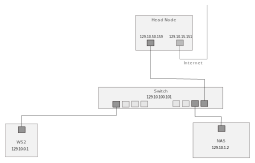
\includegraphics[scale=0.38]{qyg-c1-schem.pdf}
	\end{frame}
			
	\begin{frame}{What's a LAN?}
	A local access  network is a local configuraiton of devices that are all connected independent of the internet
	\end{frame}
	
	\begin{frame}{What's a subnet?}
	A subnet is assigned a subnet mask, with all IPs under it's mask on the subnet
	\end{frame}
			
	\begin{frame}{What's a gateway?}
	A gateway gives a LAN access to the larger internet.
	
	\end{frame}
		
	\begin{frame}{What's a DNS server?}
	A Domain Name Service (DNS) provides maps from IP to web addresses.
	
	DNS server is often set dynamically by network admins, we need to specify ourselves for subnodes.
	
	Put nameserver in file or install resolv
	\end{frame}
	
	\begin{frame}{Mounting the NAS}
	automoaund NAS on startup with /etc/fstab file
	\end{frame}
	
	\begin{frame}{What's a daemon?}
	Daemons run in the background and process requests to services that run continuously, waiting for input
	\end{frame}
	
	\begin{frame}{Systemctl}
	The system daemon controls other daemons through systemd
	
	Start and enable services via systemctl
	\end{frame}
		
	\begin{frame}{What's Slurm?}
	Slurm allows us to schedule jobs across the cluster
	\end{frame}
	
	\begin{frame}{Slurm Prerequisites}
	Munge, ntp, UIDs, slurm user + GIDs
	\end{frame}
	
	\begin{frame}{Installing Slurm}
	download, configure, make, make install, create directories and change permissions, create and copy configuration, copy daemons, reload daemons, start and enable daemons
	\end{frame}
	
	\begin{frame}{Using Slurm}
		sbatch, scontrol, sinfo, srun
	\end{frame}
	


\end{document}